\documentclass{standalone}
\usepackage{graphicx, standalone}
\usepackage[compat=1.1.0]{tikz-feynman}
\usepackage{tikz}
\usepackage{amsmath, amssymb}
\usepackage{euler}
\usepackage{fontspec}
\setmainfont{MinionPro}
\usepackage{comment}

\begin{document}

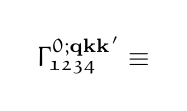
\begin{tikzpicture}[baseline=(current bounding box.center)]
	\node{$\Gamma^{0;\textbf{qkk}'}_{\mathfrak{1234}}\equiv$};
\end{tikzpicture}
%\begin{tikzpicture}[baseline=(current bounding box.center)]
%	\begin{feynman}
%		\vertex (a1);
%		\vertex[right=of a1] (b1);
%		\vertex[below=of a1] (a2);
%		\vertex[right=of a2] (b2);
		
%		\vertex[below left=-0.2em of a1] (n1) {$\mathfrak{1}$};
%		\vertex[above left=-0.2em of a2] (n2) {$\mathfrak{2}$};
%		\vertex[above right=-0.2em of b2] (n3) {$\mathfrak{3}$};
%		\vertex[below right=-0.2em of b1] (n4) {$\mathfrak{4}$};		

%		\node at ($(a1)!0.5!(b2)$) {$\Gamma^{0;\textbf{qkk}'}_{\mathfrak{1234}}$};	
		
%		\diagram* {
%			(a1) -- (b1) -- (b2) -- (a2) -- (a1),		
%		};
%	\end{feynman}
%\end{tikzpicture}
%\begin{tikzpicture}[baseline=(current bounding box.center)]
%	\node{$\equiv$};
%\end{tikzpicture}
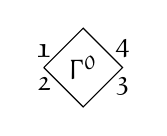
\begin{tikzpicture}[baseline=(current bounding box.center)]
	\coordinate (a1) at (0,0);
	\coordinate (b1) at (0.5,0.5);
	\coordinate (b2) at (0.5,-0.5);
	\coordinate (c1) at (1,0);
	
	\node[above=0em of a1] (n1) {$\mathfrak{1}$};
	\node[below=0em of a1] (n2) {$\mathfrak{2}$};
	\node[below=0em of c1] (n3) {$\mathfrak{3}$};
	\node[above=0em of c1] (n4) {$\mathfrak{4}$};
	
	\node at ($(a1)!0.5!(c1)$) {$\Gamma^{0}$};
	
	\draw (a1) -- (b1) -- (c1) -- (b2) -- (a1);
\end{tikzpicture}
\begin{tikzpicture}[baseline=(current bounding box.center)]
	\node{$=$};
\end{tikzpicture}
\raisebox{1mm}{
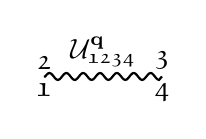
\begin{tikzpicture}[baseline=(current bounding box.center)]
	\begin{feynman}
		\vertex (a);
		\vertex[right=0.75cm of a] (b);
		\vertex[right=0.75cm of b] (c);
		
		\vertex[below=-0.1em of a] (n1) {$\mathfrak{1}$};
		\vertex[above=-0.1em of a] (n2) {$\mathfrak{2}$};
		\vertex[above=-0.1em of c] (n3) {$\mathfrak{3}$};
		\vertex[below=-0.1em of c] (n4) {$\mathfrak{4}$};	
		
		\vertex[above=0em of b] (u) {$\mathcal{U}^{\textbf{q}}_{\mathfrak{1234}}$};
		
		\diagram* {
			(a) -- [photon, thick] (c),		
		};
	\end{feynman}
\end{tikzpicture}}
\begin{tikzpicture}[baseline=(current bounding box.center)]
	\node{$-$};
\end{tikzpicture}
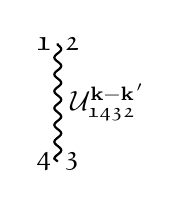
\begin{tikzpicture}[baseline=(current bounding box.center)]
	\begin{feynman}
		\vertex (a);
		\vertex[below=0.75cm of a] (b);
		\vertex[below=0.75cm of b] (c);
		
		\vertex[left=-0.1em of a] (n1) {$\mathfrak{1}$};
		\vertex[left=-0.1em of c] (n2) {$\mathfrak{4}$};
		\vertex[right=-0.1em of c] (n3) {$\mathfrak{3}$};
		\vertex[right=-0.1em of a] (n4) {$\mathfrak{2}$};	
		
		\vertex[right=0.1em of b] (u) {$\mathcal{U}^{\textbf{k}-\textbf{k}'}_{\mathfrak{1432}}$};
		
		\diagram* {
			(a) -- [photon, thick] (c),		
		};
	\end{feynman}
\end{tikzpicture}

\end{document}